\documentclass[12pt,a4paper,twoside]{report}

\usepackage{lectures}

\begin{document}
\pagestyle{fancyplain}

\begin{titlepage}
\begin{center}
\vspace*{1in}
{\LARGE \sffamily Numerické metody v astrofyzice}
\par
\vspace{1.5in}
{\large Viktor Votruba, Zdeněk Janák}
\par
\vfill
\par
\vspace{0.5in}
Přírodovědecká fakulta, sekce fyzika
\par
\vspace{0.5in}
Masarykova univerzita Brno
\par
\vspace{0.5in}
\today
\end{center}
\end{titlepage}

\thispagestyle{empty}
\begin{figure}[t!]
\begin{flushright}
\scalebox{0.85}{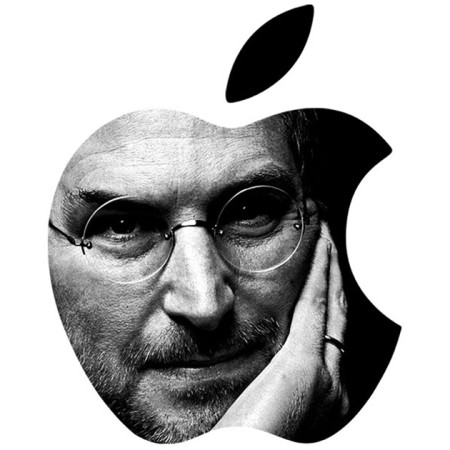
\includegraphics{steve_jobs.jpg}}
\end{flushright}
\end{figure}
\begin{verbatim}





What a computer is to me is the most remarkable tool that we have ever
come up with. It's the equivalent of a bicycle for our minds.
                  
		                                   Steve Jobs


\end{verbatim}

\tableofcontents
\thispagestyle{empty}

\chapter{Úvod}
TBD

\chapter{Jak pulsují hvězdy}

\section{Numerické řešení obyčejných diferenciálních rovnic}

S nutností řešit obyčejné diferenciální rovnice se můžeme setkat na každém kroku již během studií fyziky. Když pomineme
učebnicové případy, většinu z nich nelze řešit analyticky a musíme se uchýlit k numerickým metodám. V následující kapitole si ukážeme nejběžněji používané metody pro jejich řešení, které jsou součástí mnoha numerických knihoven v různých programovacích jazycích, včetně jazyka PYTHON. 

Nejprve se zaměříme na obyčejné diferenciální rovnici I. řádu

\begin{equation}
\label{math:ode_1order}
\deriv{y(x)}{x} = f(x,y),
\end{equation}

závěry a zkušenosti pak zobecníme na soustavu $N$ obyčejných diferenciálních rovnic I. řádu

\begin{equation}
\label{math:ode_set_1order}
\deriv{\vec{y}}{x} = \vec{f}(x,\vec{y}),
\end{equation}

kde $\vec{y}(x) = (y_1(x),y_2(x),\dots,y_n(x))$. Je třeba si uvědomit, že se nejdá o žádné omezení. Diferenciální rovnice vyšších řádů je vždy možné nahradit soustavou rovnic 1.řádu. Dále se omezíme na řešení počátečních úlohy ({\it Cauchyho úlohy}), kde k diferenciálním rovnicím máme ještě specifikované počáteční podmínky, přičemž hledáme řešení této rovnice na nějakém intervalu $x \in <a,b>$. Počáteční podmínky v případě 
(\ref{math:ode_1order}) jsou dány $y(x_0) = y_0$ , nebo v případě soustavy rovnic (\ref{math:ode_set_1order}) $\vec{y}_0 = (y_1(x_0),y_2(x_0),\dots,y_n(x_0))$.

Základem řešení rovnice  (\ref{math:ode_1order}) je její diskretizace. Spočívá v nahrazení spojitého průběhu funkce, jejich derivací i nezávislé proměnné veličiny sadou diskrétních bodů. Vytvoříme na intervalu $<a,b>$ síť ekvidistantních bodů, kterou aproximuje spojitou nezávislou veličinu $x$

\begin{equation}
a = x_0 < x_1 < x_2 < \dots < x_N = b
\end{equation}

Předpoklad ekvidistantních bodů není nutný, nicméně je pro běžné úlohy velmi častý a celou situaci zjednodušuje.

\subsection{Jednokrokové metody}
 S pomocí této sítě aproximujeme potřebnou derivaci a stačí nám k tomu Taylorův rozvoj. Taylorův rozvoj funkce $y$ v bodě $x+h$

\begin{equation}
y(x+h) = y(x)+{\deriv{y}{x}}h+{\frac{\rm d^2}y}{{\rm d}x^2}h^2+\dots
\end{equation}

kde $h$ je malý increment. Pokud zanedbáme členy druhého řádu a vyšší můžeme obratem vyjádřit aproximaci derivace s využitím sítě ekvidistantních bodů $x_k$

\begin{equation}
\deriv{y}{x} = \frac{y_{k+1}-y_{k}}{x_{k+1}-x_{k}}+O(h^) \quad k = 0,\dots, N-1,
\end{equation}

$O(h^2)$ značí chybu druhého řádu, index $k$ značí hodnotu funkce $y$ odpovídající diskrétní hodnotě proměnné $x_k$. Dosazením do rovnice (\ref{math:ode_1order}) a drobnou úpravou dostáváme

\begin{equation}
y_{k+1} = y_{k}+f(x_k,y_k)h_k \quad {\text{kde}} \quad x_{k+1}=x_k+h
\end{equation}

Tato jednoduchá metoda numerického řešení ODE se nazýva {\it Eulerova} metoda. Vzhledem k tomu, že jsme v během odvozování v Taylorově rozvoje zanedbali členy druhého řádu, jedná se o méně přesnou metodu prvního řádu. Metoda sama patří mezi {\it jednokrokové metody}, protože k závisí na informaci jednoho bodu. Přesněji řečeno, k tomu abychom určily další bod funkce $y_{k+1}$ stačí nám k tomu informace z bodu $y_k$.

\subsection{Vícekrokové metody}
Nevýhodou předchozí zmíněné metody pro řešení ODE je její přesnost. Abychom docílili vyšší přesnosti museli bychom v Taylorově rozvoji použít více členů
\begin{equation}
y(x+h) = y(x)+\deriv{y}{x}h+\frac{1}{2}\frac{{\rm d}^2 y}{{\rm d} x^2}h^2+\frac{1}{6}\frac{{\rm d}^3 y}{{\rm d} x^3}h^3+\dots
\end{equation}

Tím však vyvstává problém, protože v diskretní reprezentaci pro metodu druhého řádu vyvstává nutnost určení derivace vyšších řádů. Konkrétně v našem případě druhého řádu

\begin{equation}
\label{math:taylor_2order_runge}
y_{k+1} = y_{k} + \left.\deriv{y}{x}\right|_{k}
          h_k + \frac{1}{2} \left.\frac{{\rm d}^2 y}{{\rm d}x^2}\right|_{k} h_{k}^2
\end{equation}

S použitím pravidla pro derivaci složené funkce, můžeme pro diferenciaci $\deriv{y}{x}=f(x,y)$ psát

\begin{equation}
\frac{{\rm d}^2 y}{{\rm d}x^2} = f_x(x,y)+f_y(x,y) \deriv{y}{x} = f_x(x,y)+f_y(x,y) f(x,y)
\end{equation}

následně využijeme Taylorův rozvoj pro funkci dvou proměnných, s
pomocí které se budeme snažit vyjádřit druhou derivaci  

\begin{equation}
f(x+h,y+hf) = f(x,y)+h \frac{{\rm d}f}{{\rm d}x}+h\frac{{\rm d}f}{{\rm d}y}f+O(h^2)
\end{equation}

skombinováním obou rovnic dostáváme rovnici

\begin{equation}
\frac{{\rm d}f}{{\rm d}x}+h\frac{{\rm d}f}{{\rm d}y}f =
\frac{f(x+h,y+hf)-f(x,y)}{h}+O(h^2)
\end{equation}

Aproximaci druhé derivace s použitím diskrétní reprezentace využijeme
pro úpravu (\ref{math:taylor_2order_runge})

\begin{eqnarray}
y_{k+1} = y_k+f(x_k,y_k)h_k+\frac{f(t_k+h_k,y_k+h_k
  f(x_k,y_k))}{2h_k}h_k^2= \\
y_k+\frac{f(x_k,y_k)+f(x_k+h_k,y_k+h_k f(x_k,y_k))}{2}h_k
\end{eqnarray}

Už se blížíme k finálnímu výrazu, stačí jenom použít substituci

\begin{eqnarray}
k_1 = f(x_k,y_k)h_k \\
k_2 = f(x_k+h_k,y_k+k_1)h_k
\end{eqnarray}


\section{Jak pulsují hvězdy}
V reálné praxi astrofyzika se nutností řešení diferenciláních rovnic
setkává prakticky na každém kroku. Problémy nebeské mechaniky,
určování pohybu těles ve sluneční soustavě, teorii hvězdných atmosfér,
hvězdné stavby a mnohé další. My si jako ilustrační příklad vezmeme
nám blízký problém hvězdných pulsací. Z kurzu {\it Základů astronomie}
si určitě vzpomínáte, že některé hvězdy nezůstávají ve hydrostatické
rovnováze, ale namísto toho hvězdná obálka rozpíná a smršťuje - pulzuje.

Uvedem si teď jednoduchý model pulsující hvězdy - cefeidy, který však vede k poměrně 
přesným závěrům , zejména ve vztahu k periodě. Model se skládá z centrálního bodu reprezentující celou hvězdu o hmotnosti 
$M$, která je obklopena tenkou sféricky symetrickou obálkou o hmotnosti $m$ a poloměru $R$, která reprezentuje povrch hvězdy.
Vnitřek hvězdy je vyplněn plynem se zanedbatelnou hmotností a tlakem, který kompenzuje přitažlivý gravitační vliv centrální hvězdy na obálku. S použitím Newtonových rovnic můžeme psát

\begin{equation}
m\frac{{\rm d}^2 R}{{\rm d} t^2} = -\frac{GMm}{R^2}+4\pi R^2 P.
\end{equation}

kterou dále přepíšeme na soustavu

\begin{eqnarray}
\label{math:oscil_set_pressure}
\deriv{R}{t} = v \\
\deriv{v}{t} = -\frac{GM}{R^2} + 4\pi R^2 P/m.
\end{eqnarray}

Ještě se musíme vypořádat s tlakem, poslouží nám stavová rovnice, kdy budeme předpokládat, že oscilace od rovnovážné polohy dané poloměrem $R_0$ jsou adiabatické, tedy platí vztah

\begin{equation}
PV^{\gamma} = konst. \rightarrow {\quad} P_0 V_0^{\gamma} = P V^{\gamma}
\end{equation}

S použitím vztahu pro objem plynu v kouli $V = \frac{4}{3}\pi R^3$, můžeme dále psát

\begin{equation}
P_0 R_0^3 = P R^3 \rightarrow {\quad} P = P_0 \left(\frac{R_0}{R}\right)^{3\gamma}
\end{equation}

Dosazením do soustavy (\ref{math:oscil_set_pressure}) dostáváme finální podobu soustavu obyčejných diferenciálních rovnic popisujícich hradiální hvězdné pulsace

\begin{equation}
\label{math:oscil_final_set}
\deriv{R}{r} = v \\
\deriv{v}{t} = -\frac{GM}{R^2}+4\pi R^2 \frac{P_0}{m} \left(\frac{R_0}{R}\right)^{3\gamma}
\end{equation}

Tuto soustavu budeme řešit numericky, je však ještě třeba ji doplnit hodnoty parametrů a počáteční podmínky. Naší modelovou hvězdou bude hvězda 
$\delta$ Cep

\chapter{Základy řešení parciálních diferenciálních rovnic}

Zavzpomíname-li na základní kurzy matematické analýzy, jistě si vzpomene, jak 
nesnadné je analytické řešení parciálních diferenciálních rovnic, pokud vůbec lze 
řešení najít. Když pomineme učebnicové příklady (za zmínku stojí například vlnová 
rovnice), stojíme většinou před neřešitelným problémem. Naštestí pro nás ale ne pro 
fyziku obecně, pomocnou ruku nám podá numerické řešení problému a síla současné 
výpočetní techniky~-- počítače. Jak ale na to? Jak převést rovnici, kterou jsme 
dostali aplikací fyzikálních zákonů pro konkrétní problém do řeči čísel? 
Následující kapitola se vám pokusí v tom udělat trochu jasněji.

\section{Metoda konečných diferencí}

Jednou z nejpoužívanějších metod, která je zároveň vhodná pro názornou ilustraci, 
je {\it metoda konečných diferencí}. Nejedná se o nic jiného než diskrétní 
reprezentaci patřičných proměnných, funkcí a derivací definovaného problému. Zní to 
složitě ale ve skutečnosti je to velmi jednoduché a vše co k tomu budeme potřebovat 
je znalost Taylorova rozvoje funkce. Názorně si to ilustrujeme na jednoduché 
rovnici

\begin{equation}
\frac{\partial u}
	 {\partial t} + v \frac{\partial u}
	                       {\partial x} = D \frac{\partial^2 u}
	                                             {\partial 	x^2}
\label{rovnice}
\end{equation}

zahrnující v sobě jak difúzní $D\frac{\partial^2 u}
                                      {\partial x^2}$,
tak advekční člen $v\frac{\partial u}
                          {\partial x}$.                          
Funkce $u(x, t)$ nám udává $x$-ovou hodnotu rychlosti. Numerický přístup řešení 
této rovnice spočívá v reprezentaci $u$ souborem diskrétních hodnot $u_{i}$ v 
bodech diskrétní sítě

$$
x_0, x_1, x_2, \dots, x_i, \dots, x_N \quad (x_0 < x_1 < x_2 \dots < x_N)
$$

Na první pohled je patrné, že s rostoucím počtem bodů sítě, se bude naše 
reprezentace blížit skutečné, které bychom dosáhli pro $N = \infty$.

\subsection*{Prostorové derivace}

S touto reprezentací se můžeme dále pustit do aproximací prostorových derivací. K 
tomu využijeme Taylorova rozvoje okolo bodu $u_i$ pro hodnotu v bodě $u_{i+1}$. 
Směle můžeme psát

\begin{equation}
u_{i+1} = u_{i} +
  \left( \frac{\partial     u}{\partial   x} \right)_{i} \Delta x
+ \left( \frac{{\partial}^2 u}{\partial x^2} \right)_{i} \frac{(\Delta x)^2}{2}
+ \left( \frac{{\partial}^3 u}{\partial x^3} \right)_{i} \frac{(\Delta x)^3}{6}
+ \dots
\label{FF}
\end{equation}

Obdobně pro hodnotu $u_{i-1}$

\begin{equation}
u_{i-1} = u_{i}
- \left( \frac{\partial     u}{\partial   x} \right)_{i} \Delta x 
+ \left( \frac{{\partial}^2 u}{\partial x^2} \right)_{i} \frac{(\Delta x)^2}{2}
- \left( \frac{{\partial}^3 u}{\partial x^3} \right)_{i}\frac{(\Delta x)^3}{6}
+ \dots
\label{FB}
\end{equation}

Z Taylorova rozvoje můžeme jednoduše vyjádřit vztah pro derivaci v daném bodě $i$ 
pomocí hodnot např. $u_{i}$ a $u_{i+1}$ (nebo také $u_{i}$ a $u_{i-1}$)

\begin{equation}
\left( \frac{\partial u}{\partial x} \right)_{i}
= \frac{u_{i+1}-u_{i}}{\Delta x}
- \left( \frac{{\partial}^2 u}{\partial x^2} \right) \frac{\Delta x}{2}
- \left( \frac{{\partial}^3 u}{\partial x^3} \right) \frac{(\Delta x)^2}{6}
+ \dots
\end{equation}

Tím se dostaváme k určení prvních derivací podle prostorové souřadnice, rozlišujeme

\begin{tcolorbox}[title=Diference I. řádu - první derivace]
\begin{itemize}
    \item{ {\bf Prostorové diference (vpřed) FDS}
\begin{equation}
  \left( \frac{\partial u}{\partial x}\right)_{i}
= \frac{u_{i+1}-u_{i}}{\Delta x}+O(\Delta x)
\label{FD}
\end{equation}}
    \item{ {\bf Prostorové diference (dozadu) BDS}
\begin{equation}
  \left( \frac{\partial u}{\partial x}\right)_{i}
= \frac{u_{i}-u_{i-1}}{\Delta x} + O(\Delta x)
\label{BD}
\end{equation}}
\end{itemize}
\end{tcolorbox}

Vidíme tak, že první prostorové derivace naší funkce můžeme jednoduše vyjádřit ze 
znalostí hodnot funkce $u$ v diskrétních bodech $i-1,i,i+1$, v závislosti na 
zvoleném způsobu (\ref{FD}) resp. (\ref{BD}). Chyba, které se při této aproximaci 
dopouštíme, je prvního řádu, jak je patrné z Taylorova rozvoje.

V mnoha případech není však metoda prvního řádu dostatečná, je třeba použít 
přesnější metody, tedy druhého řádu. Odečtením rovnic (\ref{FF}) a (\ref{FB}) pro 
diferenci vzad a vpřed s Taylorovym rozvojem dostaneme výraz pro středovou 
diferenci (CD) s přesností druhého řádu \\

\begin{tcolorbox}[title = Diference II.řádu - první derivace]
\begin{itemize}
\item{{\bf Prostorové diference (centrální) CDS}
\begin{equation}
  \left( \frac{\partial u}{\partial x}\right)_{i}
= \frac{u_{i+1}-u_{i-1}}{2\Delta x} + O(\Delta x)^2
\label{CD}
\end{equation}}
\end{itemize}
\end{tcolorbox}

Nic nám již nebrání, abychom vyjádřili i druhé derivace. Stačí nám k tomu sečíst 
rovnice (\ref{FF}) a (\ref{FB}) a po úpravě dostáváme pro druhou derivaci 
diferenční vztah s přesností třetího řádu

\begin{tcolorbox}[title = Diference I. řádu - druhá derivace]
{\bf Diferenční vztah pro druhou derivaci}
\begin{equation}
  \left( \frac{{\partial}^2 u}{\partial x^2}\right)_{i}
= \frac{u_{i+1} - 2 u_i + u_{i-1}}{(\Delta x)^2}
\label{SecDer}
\end{equation}
\end{tcolorbox}

\subsection*{Časové derivace}

Obdobně budeme postupovat při určování časové derivace, nicméně je třeba přiznat, 
že se nám situace trochu komplikuje. Příčina změny je patrná z předchozích vzorců, 
rozdíl spočívá ve znalosti prostorových hodnot $u_i$ v daném časovém okamžiku. 
Prostorové derivace můžeme vyjádřit velmi snadno, pro časovou derivaci je třeba 
uvážit, že známé hodnoty funkce $u_i(t)$ jsou pouze ty současné (přítomnost) a z 
předchozích kroků (minulost). Hodnoty následující nám známé nejsou a je třeba je 
určit. Pro lepší pochopení si nejprve formálně vyjádříme časovou derivaci z rovnice 
(\ref{rovnice})

\begin{equation}
\frac{\partial u}{\partial t} = h(u, x, t)
\label{cas_der}
\end{equation}

Dále budeme postupovat jako pro prostorové derivace, nejprve diskretizujeme čas na 
jednotlivé kroky

$$
t_0, t_1, t_2, \dots, t_{n}, \dots, t_{M} \quad (t_0 < t_1 < t_2 \dots < t_{M})
$$

a určíme jednotlivé derivace podle stejného receptu

\begin{tcolorbox}[title=Časové diference I. řádu]
\begin{itemize}
\item{{\bf  (vpřed) FDT}
\begin{equation}
  \left( \frac{\partial u}{\partial t} \right)_{i}^{n}
= \frac{u_{i}^{n+1} - u_{i}^{n}}{\Delta t} + O(\Delta t)
\label{FD}
\end{equation}}
\end{itemize}
\end{tcolorbox}

Díky počatečním podmínkám známe v daném počátečním okamžiku všechny hodnoty $u_i$, 
pro $i=1,\dots,N$. Jak je naznačeno indexem u derivace na pravé straně, v tomto 
případě použijeme známé hodnoty z času $t=n$. Pro časovou derivaci (\ref{cas_der}) 
platí

\begin{eqnarray}
\frac{u_{i}^{n+1} - u_{i}^{n}}{\Delta t} = h(u^{n}, x^{n}, t)
\\
u_{i}^{n+1} = u_{i}^n + h^{n} \Delta{t} + O(\Delta x)
\end{eqnarray}

Tento hojně využívaný přístup je označován jako explicitní metoda konečných 
diferencí v čase směrem vpřed (FFTD). Obdobně pokud využijeme druhý způsob 
vyjádření derivace, tedy

\begin{tcolorbox}[title=Časové diference I. řádu]
\begin{itemize}
    \item{{\bf Časové diference (dozadu) BDT}
\begin{equation}
\left( \frac{\partial u}{\partial t} \right)_{i}^{n}
= \frac{u_{i}^{n}-u_{i}^{n-1}}{\Delta t} + O(\Delta t) = \|^{n+1}\, 
  \frac{u_{i}^{n+1}-u_{i}^{n}}{\Delta t} + O(\Delta t) 
\label{BD}
\end{equation}}
\end{itemize}
\end{tcolorbox}

Rozdíl oproti předchozímu způsobu vyjádření spočívá v použití neznámých hodnot z 
času $t = n+1$. Pro časovou derivaci (\ref{cas_der}) tak plyne

\begin{eqnarray}
\frac{u_{i}^{n+1}-u_{i}^n}{\Delta t} = h(u^{n+1}, x^{n+1}, t)
\\
u_{i}^{n+1} = u_{i}^n+h^{n+1}\Delta{t} + O(\Delta x),
\end{eqnarray}

která je označována jako implicitní metoda (BFTD). Zcela analogicky pak dostaneme 
obdobné vyjádření (taktéž implicitní) pokud použijeme centrální diferenční schéma 
(s přesností druhého řádu)

\begin{equation}
u_{i}^{n+1} = u_{i}^n + \frac{(h^{n+1} + h^{n})}{2} \Delta{t} + O(\Delta x)^2
\end{equation}

O tom, který ze způsobu vyjádření je lepší lze vést dlouhé diskuze, každý z těchto 
způsobů má své výhody a nevýhody, ať už z hlediska výpočetních nároků a nebo 
stability.

Nyní je již vše připraveno pro převod (\ref{rovnice}) do diskrétního schématu. Pro 
náš ilustrační případ zvolme pro časovou derivaci FD diferenci a CD pro advekční 
člen, druhá derivace je dána vztahem (\ref{SecDer}). Dostáváme výraz

\begin{equation}
     \frac{u_{i}^{n+1} - u_i^{n}}{\Delta t}
= - v \frac{u_{i+1}^n - u_{i-1}^n}{2\Delta x}
  + D \frac{u_{i+1}^n - 2 u_i^n+u_{i-1}^n}{(\Delta x)^2}
\end{equation}

který ještě přeuspořádáme do podoby numerického schématu (označovaného jako FTCS), 
abychom neznámé veličiny měli na leve straně a známe na pravé straně

\begin{equation}
u_{i}^{n+1} 
= u_i^{n} 
- \frac{1}{2} \frac{v \Delta t}{\Delta  x}(u_{i+1}^n - u_{i-1}^n)
+ D \frac{\Delta t}{(\Delta x)^2}(u_{i+1}^n - 2 u_{i}^{n} + u_{i-1}^n)
\label{simplefinal}
\end{equation}

Je patrné, že způsob, jakým lze původní rovnici přepsat (\ref{rovnice}) do 
diferenčního schématu není jednoznačný, máme nepřeberné množství možností 
explicitních i implicitních způsobů, které se navzájem liší výpočetní náročností, 
složitostí i stabilitou. V následujících odstavcích se seznámíme s 
nejpouživanějšími metodami.

\section{Nejjednodušší numerická schémata}

\subsection*{Laxova metoda}

Je jednou z nejjednoduších metod, hojně využivanou v numerické hydrodynamice. 
Dostaneme ji nahrazením $u_i^{n}$ v časové derivaci v rovnici (\ref{simplefinal}) 
průměrnou hodnotou určenou z jejich sousedů

$$
u_{i}^{n} \approx \frac{(u_{i+1}^{n} + u_{i-1}^n)}{2}
$$

Obdržíme Laxovo diferenční schéma

\begin{equation}
u_{i}^{n+1} 
=   \frac{1}{2}(u_{i+1}^{n}+u_{i-1}^{n})
-   \frac{1}{2}\frac{v\Delta t}{\Delta x}(u_{i+1}^n-u_{i-1}^n)
+ D \frac{\Delta t}{(\Delta x)^2}(u_{i+1}^n - 2 u_{i}^{n} + u_{i-1}^n)
\end{equation}

\subsection*{Upwind schéma }

Zvolené schéma volí jiný přístup, respektuje fyzikální podstatu problému, jinými 
slovy respektruje směr šíření proudu (tedy informace) v advekčním členu rovnice 
(\ref{rovnice}). Místo použití CD prostorové diference pro advekční člen se použije 
buď FD pro případ záporné advekční rychlosti$ v < 0$, nebo BD v případě kladné 
advekční rychlosti $v>0$. Výsledné schéma

\begin{eqnarray}
  u_{i}^{n+1}
= u_{i}^{n}
+ D\frac{\Delta t}{(\Delta x)^2}(u_{i+1}^n - 2 u_{i}^{n} + u_{i-1}^n)
-
\begin{cases}
    \frac{v\Delta t}{\Delta x}(u_{i}^n - u_{i-1}^n) \quad v > 0
    \\
    \frac{v\Delta t}{\Delta x}(u_{i+1}^n - u_{i}^n) \quad v < 0
\end{cases}
\label{upwind}
\end{eqnarray}

\subsection*{Crank-Nicholson}

Nemusíme se však omezit pouze na explicitní metody. Znamým příkladem implicitní 
metody je Crankovo-Nicholsonovo schéma, kde pro výpočet použijeme hodnoty v čase 
$t$ a $t+\Delta$ a to tak, že pro stanovení výsledné hodnoty použijeme průměr obou 
hodnot. Rovnici přepíšeme (\ref{rovnice}),

\begin{eqnarray}
  u_{i}^{n+1}
= u_i^{n}
-   \frac{1}{2}\frac{v\Delta t}{\Delta x}
    \left( \frac{1}{2}(u_{i+1}^{n+1} + u_{i+1}^{n})
-   \frac{1}{2}(u_{i-1}^{n+1} + u_{i-1}^{n}) \right)
\\
+ D \frac{\Delta t}{(\Delta x)^2}
    \left( \frac{1}{2}(u_{i+1}^{n+1} + u_{i+1}^n)
-   \frac{1}{2}(2 u_{i}^{n+1} + 2u_{i}^n)
+   \frac{1}{2}(u_{i-1}^{n+1} + u_{i-1}^n) \right)
\end{eqnarray}

a následně ještě schéma upravíme

\begin{eqnarray}
u_{i}^{n+1} & = & u_i^{n}
- \frac{1}{4}\frac{v\Delta t}{\Delta x}
  (u_{i+1}^{n+1} - u_{i-1}^{n+1} + u_{i+1}^{n} - u_{i-1}^n)
  \\
  \nonumber & + & D \frac{\Delta t}{(\Delta x)^2}
  \frac{1}{2}(u_{i+1}^{n+1}-2u_{i}^{n+1}+u_{i-1}^{n+1}+u_{i+1}^n-2u_i^n+u_{i-1}^n)
\label{crank_1}
\end{eqnarray}

Vidíme, že na rozdíl od předchozích případů nám neznámé hodnoty funkce 
$u_j^{n+1}$ v diskrétních bodech $j$ vystupují i na pravé straně. Toto schéma 
vede v tomto případě k řešení soustavy (ne)linearních rovnic (v případě nelinearity 
nutno linearizovat - například Burgersova rovnice). Pokud však $v=0$, dostáváme 
difůzní rovnici a lineární soustavu. Soustavu rovnic nejprve přepíšeme tak, že 
všechny neznáme veličiny převedeme na levou stranu. Označme

\begin{eqnarray}
\sigma = \frac{D\Delta t}{2\Delta x^2} \\
\rho   = \frac{1}{4}\frac{v\Delta t}{\Delta x}
\end{eqnarray}

pak můžeme psát pro rovnice (\ref{crank_1})

\begin{equation}
  u_{i-1}^{n+1}(-\sigma-\rho) + u_i^{n+1}(1+2\sigma) + u_{i+1}^{n+1}
= u_{i-1}^n(\sigma+\rho) + u_i^{n}(1-2\sigma) + u_{i+1}^{n}(\sigma-\rho)
\end{equation}

V maticovém formalismu můžeme rovnice přepsat následovně s použitím substituce
$A = - (\sigma+\rho)$, $B = (1+2\sigma)$, $C = (\rho-\sigma)$

\begin{equation}
\begin{pmatrix}
B & C & 0 & \cdots & \cdots & 0 \\
A & B & C & \ddots & \ddots & \vdots \\
0 & A & B & \ddots & \ddots & \vdots \\
\vdots & \ddots & \ddots & \ddots & \ddots & 0\\
\vdots & \ddots & \ddots & A & B & C \\
0 & \cdots & \cdots & 0 & A & B 
\end{pmatrix}
\begin{pmatrix}
u_1 \\ u_2 \\ \vdots \\ \\ \vdots \\ u_{M}
\end{pmatrix}
=
\begin{pmatrix}
R_1 \\ R_2 \\ \vdots \\ \\ \vdots \\ R_M
\end{pmatrix}
\end{equation}

Vektor pravých stran je dán vztahem

\begin{equation}
R_i = u_{i-1}^n(\sigma+\rho) + u_i^n(1-2\sigma)
    + u_{i+1}^n(\sigma-\rho) \quad (i \neq 1,M)
\end{equation}

Pro případ hodnoty $R_0, R_M$, je nutné si uvědomit, že hodnota funkce 
$u_{0}^{n+1}$ a $u_{M+1}^{n+1}$ je známa díky počatečním podmínkám, konkrétně

\begin{eqnarray}
u_{0}^{n+1} & = & u_{0}^{n} \\
u_{M+1}^{n+1} & = & u_{M+1}^{n} 
\end{eqnarray}

\section{Numerické testy}

\chapter{Numerické simulace hvězdného větru}

V předcházející kapitole jsme se stručně seznámili se způsobem, kterým lze úspěšně parciální diferenciální rovnice převést na řešitelný numerický problém. Studovali jsme je na jednotlivých zjednodušených typech parciálních diferenciálních rovnic, které však již v některých aspektech odráželi vlastnosti hydrodynamických rovnic. Nyní jsme vlastně již jen krůček od sestavení vlastního hydrodynamického kódu, který budeme moci použít pro studium praktického astrofyzikálního problému. V~této kapitole probereme základní pojmy, veličiny a rovnice z~klasické hydrodynamiky potřebné k~sestavení rovnic popisujících hvězdný vítr. Zvolená symetrie popisu koresponduje s~předpokládanou symetrií hvězdného větru. Pochopení matematického popisu hydrodynamiky je nezbytným krokem při sestavování vlastního kódu. V~další části této kapitoly se pak již zaměříme na numerické řešení těchto rovnic, metodu výpočtu a další aspekty, které je nutné znát pro tvorbu kódu. Na závěr si sestavíme co nejjednoduší hydrodynamický kód, který použijeme pro simulaci dvou nejznámějších typů hvězdného větru, slunečního a zářením hnaného větru horkých hvězd.
\section{Základní rovnice hydrodynamiky}
K~popisu pohybu kontinua můžeme použít dva alternativní přístupy, Eulerův popis a Langrangeův popis. V~Eulerově popisu je pohyb popsán vůči pevnému souřadnicovému systému (ne nutně inerciálnímu). Hydrodynamické rovnice jsou potom parciální diferenciální rovnice vzhledem k~prostoru a času, popisující vývoj jednotlivých hydrodynamických veličin. Naproti tomu v~Lagrangeově popisu je celé kontinuum rozděleno na určité elementární části objemu a je sledován pohyb každé této elementární části. Oba dva tyto přístupy mají své výhody a nevýhody. V~našem popisu a kódu se omezíme na první, tedy Eulerův přístup.

Nejprve zavedeme značení jednotlivých hydrodynamických veličin, kterého se budeme držet v~celém dalším textu. Základními hydrodynamickými veličinami jsou skalární hustota $\rho$, tlak $p$, vektorová rychlost elementu kontinua $\vec{v}$ a vnitřní energie plynu $U$. Tyto veličiny jsou vzájemně svázány pomocí hydrodynamických rovnic. Dále se v~našem přístupu omezíme na ideální tekutinu, nebudeme tedy započítávat vazkost tekutiny. To je v~případě drtivé většiny astrofyzikálních aplikací zcela oprávněná aproximace. V~takovém případě lze kontiunum popsat Eulerovými rovnicemi: rovnicí kontinuity, rovnicí pro hybnost a rovnicí pro energii. Obecný tvar rovnice kontinuity je podle {\citep{Landau}}
\begin{eqnarray}
		\frac{\partial{\rho}}{\partial{t}}+{\rm div}({\, \rho \vec v})=0.
		\label{konti}
\end{eqnarray} 
Obecný tvar rovnice pro hybnost za předpokladu gravitačního zrychlení $\vec{g}_*$ a 
zářivého zrychlení $\vec{g}_{\rm rad}$, lze psát 
\begin{eqnarray}
	\label{hybnost}
	\frac{\partial \vec{v}}{\partial{t}}+(\vec{v}.\nabla )\vec{v}
		+\frac{\nabla p}{\rho} = \vec{g}_*+\vec{g}_{\rm rad}.
\end{eqnarray}
Obecný tvar rovnice pro energii je dán
	\begin{eqnarray}
	\label{energie}
		\frac{\partial }{\partial{t}}\left(\frac{1}{2}v^2+\rho U\right)-{\rm div}\left(\rho\vec{v}(\frac{1}{2}v^2+H)\right)=0,
	\end{eqnarray}
kde $U$ značí vnitřní energii plynu a $H$ entalpii. V~rámci naší problematiky rovnici pro energii nebudeme nadále uvažovat. Pro jednoduchost budeme uvažovat pouze izotermické procesy (pokud bychom však chtěli započítat realističtější neizotermické procesy, je  níže uvedený postup analogický). V~rámci této aproximace ještě doplníme soustavu o~stavovou rovnici ideálního plynu
\begin{equation}
\label{staveq}
p=a^2\rho,
\end{equation}
kde $a$ značí rychlost zvuku a v~případě ideálního plynu závisí na teplotě podle vztahu
\begin{equation}
\label{soundspeed} 
a=\sqrt{\frac{k_B T}{\mu m_H}}.
\end{equation}
$k_B=1.3807\, .10^{-16}$[erg K$^{-1}$] je Boltzmannova konstanta, $m_{H}$ je hmotnost atomu vodíku a $\mu_{m}$ je střední molekulová hmotnost plynu. Přesný výpočet $\mu$ je poměrně komplikovaný a závisí na určení stupně ionizace všech chemických elementů v~plynu.
\section{Základy numerické dynamiky tekutin}
\subsection{Konzervativní schéma}
Hydrodynamické rovnice lze numericky formulovat jak v Langrangeově formalismu, tak v Eulerově formalismu. Základní vlastností Lagrangeova přístupu je, že celková hmota se zachovává. Pro numerické schéma v Eulerově formalismu to nemusí být obecně pravda. Je však možne Eulerovy rovnice do konzervativní formy přepsat. Jaký je tedy v tom rozdíl ? Uvažme derivaci z rovnice kontinuity
\begin{equation}
\label{conserve_example}
\frac{\partial \rho u}{\partial x},
\end{equation}
kterou diskretizujeme následujícím způsobem,
\begin{equation}
\label{con_1}
\frac{\partial \rho u}{\partial x}=\frac{(\rho u)_{i}-(\rho u)_{i-1}}{\Delta x}.
\end{equation}
Můžeme však také derivaci (\ref{conserve_example}) rozepsat
\begin{equation}
\rho \frac{\partial u}{\partial x}+u\frac{\partial \rho}{\partial x}.
\end{equation}
Což s použitím stejné numerické aproximace jako v případě (\ref{con_1}) vede
\begin{equation}
\label{con_2}
\rho \frac{\partial u}{\partial x}+u\frac{\partial \rho}{\partial x} = \rho_i\frac{u_i-u_{i-1}}{\Delta x}+u_i\frac{\rho_i-\rho_{i-1}}{\Delta x},
\end{equation}
Vidíme, že výsledne numerické schéma (\ref{con_1}) a (\ref{con_2}) aproximované derivace (\ref{conserve_example}) není stejné, ač vychází ze stejné 
rovnice a stejného numerického přístupu. Ale zachovává vztah (\ref{con_1}) skutečně hmotu na rozdíl od (\ref{con_2})? Abychom se o tom přesvědčili, stačí 
sečíst výsledný vztah přes všechny body sítě.  Zvolme pro jednoduchost případ sítě se čtyřmi body, dostáváme
\begin{equation}
\label{conserve_form_expl_1}
\frac{(\rho u)_{1}-(\rho u)_{0}}{\Delta x}+\frac{(\rho u)_{2}-(\rho u)_{1}}{\Delta x}+\frac{(\rho u)_{3}-(\rho u)_{2}}{\Delta x}
\end{equation}
ze kterého je ihned patrné, že zbývají pouze členy na okraji $i=0$ a $i=3$, tedy pouze na tom kolik hmoty vchází dovnitř a kolik vychází ven. V případě
druhém (\ref{con_2}) je situace komplikovanější
\begin{equation}
\label{conserve_form_expl_2}
\rho_1\frac{u_1-u_{0}}{\Delta x}+u_1\frac{\rho_1-\rho_{0}}{\Delta x}+\rho_2\frac{u_2-u_{1}}{\Delta x}+u_2\frac{\rho_2-\rho_{1}}{\Delta x}+\rho_3\frac{u_3-u_{2}}{\Delta x}+u_3\frac{\rho_3-\rho_{2}}{\Delta x}
\end{equation}
jednotlivé vnitřní členy se nevyruší, pokud přidáme další bod sítě přidáme i další člen a výsledná suma je větší. Nelze tedy hovořit o zachování hmoty.

V praxi je použití konzervativního schématu velkou výhodou, poněvadž respektuje fyzikální podstatu problému. Navíc oproti nekonzervativním schématům vykazují větší stabilitu a přesnost v případě existence rázových vln během studovaného procesu. Eulerovy hydrodynamické rovnice (rovnici pro energii pro jednoduchost neuvažujeme) tedy přepíšeme do konzervativního tvaru
\begin{equation}
\label{euler_conserve}
\vec{u}_t+\vec{F}(\vec{u})_{x} = 0.
\end{equation}
kde
\begin{equation}
\label{vector_form}
\vec{u} = \begin{pmatrix}
		\rho \\
		\rho v
		\end{pmatrix}\quad,\quad\vec{F}(\vec{u}) = \begin{pmatrix}
						\rho v \\
						\rho v^2 + p
					\end{pmatrix}.
\end{equation}
Abychom lépe ilustrovali výhody, které přináší tento přístup, zavedeme speciální typ sítě, který se ve spojitosti s konzervativním typem schématu často používá. Jedná se o střídavou síť ( v anglické literatuře označovanou jako {\it staggered}), ve které hustota (a další skalární veličiny) je definována ve středu výpočetní buňky, zatímco rychlost (vektorová veličina) na jejím okraji (viz. obrazek \ref{figure:grid_staggered}). S použitím konzervativního schématu Eulerových rovnic, lze pak říci, že hustota ve středu výpočetní buňky je dána tokem hmoty, přes její okraje.
\subsection{Technika oddělených toků}
\label{technikaodd}
Tato metoda, známá spíše pod svým anglickým názvem {\it flux splitting} technika \citep[stránka 415]{Hirsch2002}, umožňuje rozdělit řešení parciální diferenciální rovnice na části, kde každá část reprezentuje jeden samostatný člen z~uvažované rovnice. Schématicky zapsáno, pro dynamický systém daný rovnicí
\begin{equation}
\frac{\partial \vec{u}}{\partial t}=\mathcal{L}(\vec{u})
\label{schemasplit}
\end  {equation}
je $\vec{u}$  je reprezentováno sloupcovým vektorem (\ref{vector_form}). Operátor $\mathcal{L}(\vec{y})$ můžeme rozložit na součet částečných operátorů $\mathcal{L}(\vec{u})=\mathcal{L}_1(\vec{u})+\mathcal{L}_2(\vec{u})+\dots +\mathcal{L}_m(\vec{u})$, přičemž každý operátor představuje jeden člen z rovnice. Tedy například advekční člen, člen odpovídající tlakovým, gravitačním silám apod. Numerické řešení rovnice \eqref{schemasplit} pak obdržíme postupnou aplikací jednotlivých operátorů 
\begin{eqnarray}
\vec{u}^{n+1/m} &=&\mathcal{L}_1(\vec{u}^n,\Delta{t}), \\
\nonumber \vec{u}^{n+2/m} &=&\mathcal{L}_2(\vec{u}^{n+1/m},\Delta{t}), \\
\nonumber \vec{u}^{n+3/m} &=&\mathcal{L}_3(\vec{u}^{n+2/m},\Delta{t}), \\
\nonumber \vdots &=&\vdots, \\
\nonumber \vec{u}^{n+1} &=&\mathcal{L}_m(\vec{u}^{n+m-1/m},\Delta{t})
\end{eqnarray}

\section{Advekční člen}
Rozepíšeme Eulerovy rovnice 1D v kartézských souřadnicích a v konzervativním tvaru ({\ref{euler_conserve}) dostáváme
\begin{eqnarray}
\label{euler_expanded}
\frac{\partial{\rho}}{\partial t} + \frac{\partial{\rho v}}{\partial x} = 0 \\
\frac{\partial{\rho v}}{\partial t} + \frac{\partial{\rho v^2}}{\partial x}+\frac{\partial p}{\partial x} = 0
\end{eqnarray}
první dva členy v obou rovnicích reprezentují změnu hustoty a momentu hybnosti jako výsledek přenosu hmoty a memonetu hybnosti podél sítě. To je podstata advekčního členu, nedochází k celkové změně hmotnosti a momentu hybnosti, vyjma toho co do systému vchází a odchází v důsledku okrajových podmínek. Z numerického hlediska je však podstatné, aby ta část numerického výpočtu, která počítá advekční člen byla provedena konzistentně. Tím máme na mysli, aby advekce všech fyzikálních veličin, tedy jak hustoty, tak momentu hybnosti byly počítány stejným způsobem. Jinak řečeno, pokud dochází k přetoku hmotnostního elementu z jedné výpočetní buňky do druhé, dochází také ve stejný okamžik k přetoku momentu hybnosti. 
\begin{figure}
\centering
\scalebox{0.85}{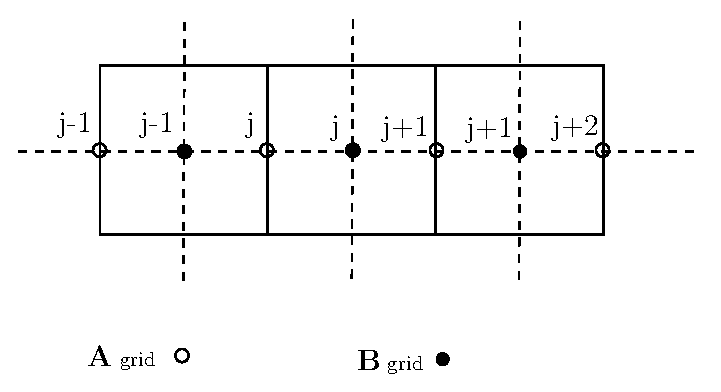
\includegraphics{grid.eps}}
\caption{\it Střídavý typ sítě, skalární veličiny jsou definováne na středu výpočetní buňky - body {\bf B}, vektorové veličiny jsou definovány na okrajích výpočetní buňky - body {\bf A}.}
\label{figure:grid_staggered}
\end{figure}
Pro ilustraci se podívejme na rovnici kontinutiy (\ref{euler_expanded}), obecné numerické schéma pro řešení této rovnice pro advekci
\begin{equation}
\rho_{B,i}^{n+1} = \rho_{B,i}^{n} - \frac{\Delta t^{n+1/2}}{\Delta x_{B,i}}(F_{i+1}-F_i) = \rho_{B,i}^n-\frac{\Delta t^{n+1/2}}{\Delta x_{B,i}^{n}}\left((\overline{\rho} v)_{i+1}-({\overline \rho} v )_{i}\right)
\end{equation}
kde 
\begin{equation}
\Delta x_{B,i} = x_{A,i+1}-x_{A,i}.
\end{equation}
Pro vysvětlenou: horní index u časového kroku je zde proto, že velikost časového kroku se během časového vývoje mění tak, aby vždy byla splněna Courantova podmínka stability. Hustota $\overline{\rho}$ vystupující v členech odpovídající toku hmoty skrze hranice výpočetní buňky, by měla co nejvíce odpovídat množství hmoty protékající skrze hranice buňky. Její hodnotu dostaneme interpolací, zaléží však na metodě, kterou zvolíme. Dále je třeba upozornit, že byla použita střídavá síť, kde skalární veličiny jsou definovány na středu výpočetní buňky (typ B) a vektorové veličiny na jejích okrajích (typ A).

Možností je více, aby však schéma bylo stabilní schéma musíme respektovat směr šíření informací skrze hranici výpočetní buňky (viz. \ref{section:upwind}}. V nejjednoduším případě stačí použít hodnotu hustoty ze středu buňky ze které přitéká hmota ({\it donor cell} schéma). Tedy například pro hraniční bod buňky $x_i$ oddělující výpočetní buňky s hustotou $\rho_{B,i-1}$ a $\rho_{B,i}$ platí pro tento postup
\begin{equation}
\overline{\rho} =
\begin{cases}
\rho_{B,i-1} \quad v_i > 0 \\
\rho_{B,i} \quad v_i < 0
\end{cases}
\end{equation}
Toto schéma však je metodou prvního řádu, není příliš přesné díky většímu vlivu numerické difůze. Mnohem přesnější metodou dostaneme, pokud do interpolované veličiny, v našem případě $\overline{\rho}$ zahrneme aproximativně průběh změny této veličiny mezi středy výpočetní buňky. Nejjednodušší možností aproximace je lineární průběh.
\subsection{VanLeerova metoda}
Podívejme se dobře na obrázek \ref{image:vanleer}, uvažme situaci na hranici buňky $x_i$. Nejjednoduší způsob, jak lineární funkcí aproximovat průběh hustoty uvnitř výpočetní buňky za předpokladu, že známe hodnotu hustoty v jejím středu by bylo použítí hodnot $\rho_{B,i-1}$ a $\rho_{B,i}$ ke stanovení směrnice přímky a tuto hodnotu použít pro stanovení průběhu v obou buňkách včetně jejich okrajů, to by však vedlo ke značně zkresleným hodnotam na krajích $x_{A,i-1}$ a $x_{A,i+1}$. Další možností by mohlo být použití průměru $\Delta\overline{\rho}_{i}$ ze směrnic určených z bodů $\rho_{B,i-1},\rho_{B,i}$ a $\rho_{B,i},\rho_{B,i+1}$ pro buňku mezi body $x_{A,i},x_{A,i+1}$ a obdobně $\Delta\overline{\rho}_{i-1}$ ze směrnic určených z bodů $\rho_{B,i-2},\rho_{B,i-1}$ pro buňku mezi body $x_{A,i-1},x_{A,i}$. Ani v tomto případě se nevyhneme problémům s existencí nereálných maxim na krajích buněk viz obrázek. S těmito obtižemi se lze vypořádat použitím vanLeerovy monotonizace. Její princip je velmi jednoduchý, nejprve určíme směrnice
\begin{equation}
\Delta\rho_{A,i} = \frac{\rho_{B,i}+\rho_{B,i-1}}{\Delta{x_{A,i}}}
\end{equation}
kde $\Delta{x_{A,i}}=0.5(\Delta x_{B,i-1}+\Delta x_{B,I})$. Pro hledanou hodnotu interpolované veličiny použijeme hodnoty, které odpovídají směru toku šíření informace. Tedy s využitím směru šíření informace
\begin{tcolorbox}[title=Advekce hustoty - VanLeer schéma]
\begin{equation}
\overline{\rho} =
\begin{cases}
 \rho_{B,i-1}+(\Delta x_{B,i-1}-v_{A,i}\Delta t)\frac{{\rm d}\rho_{B,i-1}}{2} \quad v_i > 0 \\
 \rho_{B,i}-(\Delta x_{B,i}+v_{A,i}\Delta t)\frac{{\rm d}\rho_{B,i}}{2} \quad v_i < 0
\end{cases}
\end{equation}
\end{tcolorbox}
kde směrnice přímky ${\rm d}\rho_{i-1},{\rm d}\rho_{i}$ je dána geometrickým průměrem
\begin{eqnarray}
{\rm d}\rho_{B,i-1} =\frac{2\Delta\rho_{A,i}\Delta{\rho_{A,i-1}}}{\Delta \rho_{A,i}+\Delta \rho_{A,i-1}} \\
{\rm d}\rho_{B,i} = \frac{2\Delta\rho_{A,i}\Delta{\rho_{A,i+1}}}{\rho_{A,i}+\rho_{A,i+1}}
\end{eqnarray}
pokud $\Delta\rho_{A,i}\Delta{\rho_{A,i-1}} > 0$ resp. $\Delta\rho_{A,i}\Delta{\rho_{A,i+1}} > 0$ a na druhou stranu
\begin{equation}
{\rm d}\rho_{B,i-1} = 0, \quad {\rm d}\rho_{B,i} = 0
\end{equation}
 za předpokladu, že $\Delta\rho_{A,i}\Delta{\rho_{A,i-1}} < 0$ resp. $\Delta\rho_{A,i}\Delta{\rho_{A,i+1}} < 0$.
Tento postup použijeme i na další interpolovanu veličinu v advektním členu, moment hybnosti $\overline{\rho v}$. Musíme si však uvědomit, že moment hybnosti je definován na krajích výpočetní buňky (na síti typu A) na rozdíl od hustoty. Tedy
\begin{tcolorbox}[title= Advekce momentu hybnosti - VanLeer schéma]
\begin{equation}
\overline{\vec{\rho v}} =
\begin{cases}
{\rho v}_{A,i}+(\Delta x_{A,i}-v_{B,i}\Delta t)\frac{{\rm d}(\rho v)_{A,i}}{2} \quad v_i > 0 \\
{\rho v}_{A,i+1}-(\Delta x_{A,i+1}+v_{B,i}\Delta t)\frac{{\rm d}(\rho v)_{A,i+1}}{2} \quad v_{i} < 0
\end{cases}
\end{equation}
\end{tcolorbox}
přičemž pro derivaci platí obdobně jako v předchozím případě
\begin{equation}
{\rm d}(\rho v)_{A,j} = 
\begin{cases}
\frac{{2}{\Delta (\rho v)_{B,j} \Delta (\rho v)_{B,j+1}}}{\Delta (\rho v)_{B,j}
+\Delta (\rho v)_{B,j+1}} \quad \text{pokud} \quad {\Delta (\rho v)_{B,j} \Delta (\rho v)_{B,j+1}} > 0 \\
0  \quad \text{pokud} \quad {\Delta (\rho v)_{B,j} \Delta (\rho v)_{B,j+1}} < 0
\end{cases}
\end{equation}
kde $j = {i,i+1}$.
\section{Zdrojové členy}
V předchozí části jsme se zabývali advekčním členem přítomným v Eulerových rovnicích. Zbývající $m-$ dynamických členů jako je gravitační síla, tlaková síla a další nazýváme shrnutě zdrojové členy. Tyto členy do numerického schématu zahrnujeme s pomocí techniky oddělených toků. Tedy každý člen bude zahrnut samostatně, jeden po druhém.
\begin{tcolorbox}[title=Zdrojové členy]
\begin{eqnarray}
{\rho v}_i^{n+1/m} ={\rho v}_i^{n}+\Delta t \mathcal{L}_1\\
{\rho v}_i^{n+2/m} ={\rho v}_i^{n+1/m}+\Delta t \mathcal{L}_2 \\
\nonumber \cdots \\
{\rho v}_i^{n+1} = {\rho v}_i^{n+(m-1)/m}+\Delta t \mathcal{L}_m
\end{eqnarray} 
Pro ilustraci, předpokládejme, že například $\mathcal{L}_1$ reprezentuje tlakovou sílu, pak ma operátor tvar
\begin{equation}
\mathcal{L}_1 = a^2 \frac{(\rho_{B,i}-\rho_{B,i-1})}{x_{B,i}-x_{B,i-1}}
\end{equation}
\end{tcolorbox}
Obdobně bychom postupovali při konstrukci operátory reprezentujících další zdrojové členy.
\subsection{Tvorba vlastního kódu}
\begin{figure}
\centering
\scalebox{0.65}{\includegraphics{schema.pdf}}
\caption{Schéma procesu výpočtu v hydrodynamickém kódu}
\label{figure:schema}
\end{figure}
Nyní již máme skoro všechny potřebné znalosti k tvorbě vlastního kódu. Stačí jen si tyto znalosti utřídit. Rozdělíme si náš úkol do tří základních fází: {\it přípravnou, výpočetní a výstupní}. V přípravné fázi vytvoříme střídavou síť, inicializujeme potřebné proměnné a nastavíme počáteční podmínky studovaného problému. Ve výpočetní fázi budeme provádět vlastní numerické řeěení Eulerových rovnic pro danný problém. Konkrétně vyřešíme advekční členy pro hustotu i moment hybnosti, změnu momentu hybnosti v důsledku existence zdrojových členů, aplikujeme okrajové podmínky a aktualizujeme všechny potřebné veličiny pro další krok výpočtu. Výpočet probíhá dokud doba výpočtu neodpovídá času, v kterém hledáme řešení. V závěrečné výstupní fázi určíme veličiny, vhodné ke grafickému či jinému výstupu pro další analýzu.
\section{Astrofyzikální aplikace - hvězdný vítr}
Náš hydrodynamický nebude jen pouhou hříčkou, lze jej použít ke studiu různých astrofyzikálních problémů. Jedním z takových problémů je hvězdný vítr hvězd. Mezi dva nejznámější typy hvězdného větru patří sluneční vítr a hvězdný vítr horkých hvězd. Sluneční vítr je typ hvězdného větru , ve kterém dominantní hnací složkou jsou tlakové síly v důsledku velké teploty koróny, tak jak je tomu u našeho Slunce. Naproti tomu v případě hvězdného větru horkých hvězd je hlavní hnací složkou zářivá síla, která souhrně popisuje interakci záření s hmotou. Detailní popis obou typů hvězdného větru můžeme najít například v \citep{Lamers}, popřípadě \citep{Thompson}. 

Podívejme se teď trochu podrobněji na druhý typ hvězdného větru. To proto, že musíme do hydrodynamických rovnic přidat nový zdrojový člen, konkrétně zářivá síla. Zářivá síla v CAK aproximaci je dána
\begin{equation}
\label{equation:CAK}
g_{\rm rad}= \frac{C}{r^2}\left(\frac{1}{\rho}\frac{{\rm d}v}{{\rm d}r}\right)^{\alpha}
\end{equation}  
kde $C$ označujeme jako zářivou konstantu
\begin{equation}
\label{equation:cak_constant}
C =\frac{k}{4\pi c}\frac{(\kappa_e^{\rm ref})^{1-\alpha}}{v_{\rm th}^{\alpha}}L_{*}
\end{equation} 
Hodnota CAK parametru $\alpha$ je v původní verzi \citep{A1980,} tabelována, nicméně lze použít s výhodou hodnotu $\alpha = 0.5$. 

Náš hydrodynamický kód je časově závislý, který umožňuje simulaci i časově proměnných, nicméně nás bude v případě simulace hvězdného větru stacionární, časově neproměnné řešení. To odpovída realitě, kdy základní dynamické charakteristiky hvězdného větru jsou dlouhodobě relativně stabilní. Ze všech možných stacionárních řešení se dále budeme snažit o nalezení kritického CAK řešení, což je řešení které začíná u povrchu hvězdy s podzvukovou rychlostí, prochází přes kritický CAK bod dále do nadzvukové oblasti. Detaily lze opět nalézt v \citep{Lamers}. Analyticky lze pro případ kritického CAK řešení určit rychlost ztráty hmoty
\begin{equation}
\dot{M}_{\rm CAK} = 4\pi\rho(r)v(r)r^2 = \frac{\left(k \kappa_e^{\rm ref}L_*\right)^{1/\alpha}}{\kappa_e^{\rm ref}(4\pi c)^{1/\alpha}}\frac{4\pi(GM_*(1-\Gamma_e))^{(\alpha-1)/\alpha}}{v_{\rm th}}\frac{\alpha(1-\alpha)^{1/\alpha}}{(1-\alpha)}
\end{equation}
Tuto skutečnost s výhodou využijeme při upravě rovnic do bezrozměrného tvaru. Jednoduše řečeno, neni pro nás podstatný průběh pro konkrétní hvězdu s danou hmotností, teplotou a luminositou. Zajímá nás průběh kritického řešení pro hvězdu u které je hvězdný vítr hnaný zářením. Základem je vhodná volba normalizačních konstant pro jednotku délky $R_{N}$, hmotnosti $M_{N}$ a času $S_N$. S využitím zvolených normalizačních podmínek $GM_*=1$, $R_* = 1$ a $\dot{M}_{\rm CAK}/4\pi = 1$, dostáváme 
\begin{eqnarray}
R_{N} = R_*, \\
S_{N} = \sqrt{\frac{{R_N}^3}{GM_*}},\\
M_{N} = \frac{\dot{M}_{\rm CAK}}{S_N}
\end{eqnarray}

\chapter{Optimalizace - řešení inverzních úloh}

\chapter{Jak na GIT}


\bibliographystyle{plainnat}
\bibliography{lectures}

\end{document}
